% Options for packages loaded elsewhere
\PassOptionsToPackage{unicode}{hyperref}
\PassOptionsToPackage{hyphens}{url}
\documentclass[
]{article}
\usepackage{xcolor}
\usepackage[margin=1in]{geometry}
\usepackage{amsmath,amssymb}
\setcounter{secnumdepth}{-\maxdimen} % remove section numbering
\usepackage{iftex}
\ifPDFTeX
  \usepackage[T1]{fontenc}
  \usepackage[utf8]{inputenc}
  \usepackage{textcomp} % provide euro and other symbols
\else % if luatex or xetex
  \usepackage{unicode-math} % this also loads fontspec
  \defaultfontfeatures{Scale=MatchLowercase}
  \defaultfontfeatures[\rmfamily]{Ligatures=TeX,Scale=1}
\fi
\usepackage{lmodern}
\ifPDFTeX\else
  % xetex/luatex font selection
\fi
% Use upquote if available, for straight quotes in verbatim environments
\IfFileExists{upquote.sty}{\usepackage{upquote}}{}
\IfFileExists{microtype.sty}{% use microtype if available
  \usepackage[]{microtype}
  \UseMicrotypeSet[protrusion]{basicmath} % disable protrusion for tt fonts
}{}
\makeatletter
\@ifundefined{KOMAClassName}{% if non-KOMA class
  \IfFileExists{parskip.sty}{%
    \usepackage{parskip}
  }{% else
    \setlength{\parindent}{0pt}
    \setlength{\parskip}{6pt plus 2pt minus 1pt}}
}{% if KOMA class
  \KOMAoptions{parskip=half}}
\makeatother
\usepackage{color}
\usepackage{fancyvrb}
\newcommand{\VerbBar}{|}
\newcommand{\VERB}{\Verb[commandchars=\\\{\}]}
\DefineVerbatimEnvironment{Highlighting}{Verbatim}{commandchars=\\\{\}}
% Add ',fontsize=\small' for more characters per line
\usepackage{framed}
\definecolor{shadecolor}{RGB}{248,248,248}
\newenvironment{Shaded}{\begin{snugshade}}{\end{snugshade}}
\newcommand{\AlertTok}[1]{\textcolor[rgb]{0.94,0.16,0.16}{#1}}
\newcommand{\AnnotationTok}[1]{\textcolor[rgb]{0.56,0.35,0.01}{\textbf{\textit{#1}}}}
\newcommand{\AttributeTok}[1]{\textcolor[rgb]{0.13,0.29,0.53}{#1}}
\newcommand{\BaseNTok}[1]{\textcolor[rgb]{0.00,0.00,0.81}{#1}}
\newcommand{\BuiltInTok}[1]{#1}
\newcommand{\CharTok}[1]{\textcolor[rgb]{0.31,0.60,0.02}{#1}}
\newcommand{\CommentTok}[1]{\textcolor[rgb]{0.56,0.35,0.01}{\textit{#1}}}
\newcommand{\CommentVarTok}[1]{\textcolor[rgb]{0.56,0.35,0.01}{\textbf{\textit{#1}}}}
\newcommand{\ConstantTok}[1]{\textcolor[rgb]{0.56,0.35,0.01}{#1}}
\newcommand{\ControlFlowTok}[1]{\textcolor[rgb]{0.13,0.29,0.53}{\textbf{#1}}}
\newcommand{\DataTypeTok}[1]{\textcolor[rgb]{0.13,0.29,0.53}{#1}}
\newcommand{\DecValTok}[1]{\textcolor[rgb]{0.00,0.00,0.81}{#1}}
\newcommand{\DocumentationTok}[1]{\textcolor[rgb]{0.56,0.35,0.01}{\textbf{\textit{#1}}}}
\newcommand{\ErrorTok}[1]{\textcolor[rgb]{0.64,0.00,0.00}{\textbf{#1}}}
\newcommand{\ExtensionTok}[1]{#1}
\newcommand{\FloatTok}[1]{\textcolor[rgb]{0.00,0.00,0.81}{#1}}
\newcommand{\FunctionTok}[1]{\textcolor[rgb]{0.13,0.29,0.53}{\textbf{#1}}}
\newcommand{\ImportTok}[1]{#1}
\newcommand{\InformationTok}[1]{\textcolor[rgb]{0.56,0.35,0.01}{\textbf{\textit{#1}}}}
\newcommand{\KeywordTok}[1]{\textcolor[rgb]{0.13,0.29,0.53}{\textbf{#1}}}
\newcommand{\NormalTok}[1]{#1}
\newcommand{\OperatorTok}[1]{\textcolor[rgb]{0.81,0.36,0.00}{\textbf{#1}}}
\newcommand{\OtherTok}[1]{\textcolor[rgb]{0.56,0.35,0.01}{#1}}
\newcommand{\PreprocessorTok}[1]{\textcolor[rgb]{0.56,0.35,0.01}{\textit{#1}}}
\newcommand{\RegionMarkerTok}[1]{#1}
\newcommand{\SpecialCharTok}[1]{\textcolor[rgb]{0.81,0.36,0.00}{\textbf{#1}}}
\newcommand{\SpecialStringTok}[1]{\textcolor[rgb]{0.31,0.60,0.02}{#1}}
\newcommand{\StringTok}[1]{\textcolor[rgb]{0.31,0.60,0.02}{#1}}
\newcommand{\VariableTok}[1]{\textcolor[rgb]{0.00,0.00,0.00}{#1}}
\newcommand{\VerbatimStringTok}[1]{\textcolor[rgb]{0.31,0.60,0.02}{#1}}
\newcommand{\WarningTok}[1]{\textcolor[rgb]{0.56,0.35,0.01}{\textbf{\textit{#1}}}}
\usepackage{graphicx}
\makeatletter
\newsavebox\pandoc@box
\newcommand*\pandocbounded[1]{% scales image to fit in text height/width
  \sbox\pandoc@box{#1}%
  \Gscale@div\@tempa{\textheight}{\dimexpr\ht\pandoc@box+\dp\pandoc@box\relax}%
  \Gscale@div\@tempb{\linewidth}{\wd\pandoc@box}%
  \ifdim\@tempb\p@<\@tempa\p@\let\@tempa\@tempb\fi% select the smaller of both
  \ifdim\@tempa\p@<\p@\scalebox{\@tempa}{\usebox\pandoc@box}%
  \else\usebox{\pandoc@box}%
  \fi%
}
% Set default figure placement to htbp
\def\fps@figure{htbp}
\makeatother
\setlength{\emergencystretch}{3em} % prevent overfull lines
\providecommand{\tightlist}{%
  \setlength{\itemsep}{0pt}\setlength{\parskip}{0pt}}
\usepackage{bookmark}
\IfFileExists{xurl.sty}{\usepackage{xurl}}{} % add URL line breaks if available
\urlstyle{same}
\hypersetup{
  pdftitle={Regresní analýza},
  hidelinks,
  pdfcreator={LaTeX via pandoc}}

\title{Regresní analýza}
\author{}
\date{\vspace{-2.5em}}

\begin{document}
\maketitle

\subsection{LMER model - fixní
ticker}\label{lmer-model---fixnuxed-ticker}

Všechny fixní efekty mimo modelu jsou statisicky významné. Velmi malý
efekt náhodné složky (měsíc sběru). Nízké mezní \(R^2\), nelze vypočítat
podmíněné \(R^2\) kvůli nízkému efektu měsíců.

\begin{Shaded}
\begin{Highlighting}[]
\NormalTok{subset\_args }\OtherTok{\textless{}{-}} \FunctionTok{c}\NormalTok{(}
  \StringTok{"S"}\NormalTok{,}
  \CommentTok{\#"moneyness",}
  \StringTok{"K"}\NormalTok{,}
  \StringTok{"r"}\NormalTok{,}
  \StringTok{"sigma"}\NormalTok{,}
  \StringTok{"q"}\NormalTok{,}
  \StringTok{"T"}\NormalTok{,}
  \StringTok{"am\_eu"}\NormalTok{,}
  \StringTok{"call\_put"}\NormalTok{,}
  \StringTok{"model"}\NormalTok{,}
  \StringTok{"ticker"}
\NormalTok{  )}
\NormalTok{interactions }\OtherTok{\textless{}{-}} \FunctionTok{c}\NormalTok{(}
  \CommentTok{\#"(1 | ticker)",}
  \StringTok{"(1 | snapshot\_month)"}
\NormalTok{)}

\NormalTok{rhs }\OtherTok{\textless{}{-}} \FunctionTok{paste}\NormalTok{(}\FunctionTok{c}\NormalTok{(subset\_args, interactions), }\AttributeTok{collapse =} \StringTok{" + "}\NormalTok{)}
\NormalTok{formula }\OtherTok{\textless{}{-}} \FunctionTok{as.formula}\NormalTok{(}\FunctionTok{paste}\NormalTok{(}\StringTok{"pricing\_error \textasciitilde{} "}\NormalTok{, rhs))}

\NormalTok{rmr\_relative }\OtherTok{\textless{}{-}} \FunctionTok{lmer}\NormalTok{(formula, }\AttributeTok{data =}\NormalTok{ train\_data\_rel)}
\end{Highlighting}
\end{Shaded}

\begin{verbatim}
## fixed-effect model matrix is rank deficient so dropping 1 column / coefficient
\end{verbatim}

\begin{Shaded}
\begin{Highlighting}[]
\FunctionTok{summary}\NormalTok{(rmr\_relative)}
\end{Highlighting}
\end{Shaded}

\begin{verbatim}
## Linear mixed model fit by REML. t-tests use Satterthwaite's method [
## lmerModLmerTest]
## Formula: formula
##    Data: train_data_rel
## 
## REML criterion at convergence: -1766596
## 
## Scaled residuals: 
##     Min      1Q  Median      3Q     Max 
## -6.9817 -0.3327  0.0635  0.4441  5.1644 
## 
## Random effects:
##  Groups         Name        Variance  Std.Dev. 
##  snapshot_month (Intercept) 5.208e-07 0.0007216
##  Residual                   2.746e-04 0.0165700
## Number of obs: 329512, groups:  snapshot_month, 4
## 
## Fixed effects:
##                 Estimate Std. Error         df t value Pr(>|t|)    
## (Intercept)   -3.113e-02  1.331e-03  5.360e+02 -23.389  < 2e-16 ***
## S              1.243e-05  6.012e-07  8.341e+04  20.684  < 2e-16 ***
## K             -7.506e-06  1.395e-07  3.295e+05 -53.819  < 2e-16 ***
## r              1.781e+00  2.844e-02  1.414e+05  62.616  < 2e-16 ***
## sigma         -8.096e-02  1.256e-03  5.932e+04 -64.461  < 2e-16 ***
## q             -4.741e-01  4.962e-02  3.294e+05  -9.555  < 2e-16 ***
## T              3.880e-03  4.146e-05  3.294e+05  93.593  < 2e-16 ***
## am_eueuropean -3.048e-02  1.497e-03  4.768e+04 -20.366  < 2e-16 ***
## call_putputs  -3.148e-03  6.029e-05  3.295e+05 -52.215  < 2e-16 ***
## modeluser_crr -8.143e-06  7.071e-05  3.295e+05  -0.115   0.9083    
## modeluser_mc   1.578e-05  7.070e-05  3.295e+05   0.223   0.8234    
## ticker^XDA    -1.496e-02  2.345e-03  2.352e+05  -6.377 1.80e-10 ***
## ticker^XDB     1.869e-02  2.161e-03  2.249e+05   8.649  < 2e-16 ***
## ticker^XDE     4.192e-03  1.882e-03  1.795e+05   2.228   0.0259 *  
## ticker^XDN     1.217e-02  2.013e-03  1.871e+05   6.046 1.49e-09 ***
## tickerAAPL    -1.375e-02  4.226e-04  1.776e+05 -32.535  < 2e-16 ***
## tickerAMD      1.059e-02  1.749e-04  1.085e+05  60.537  < 2e-16 ***
## tickerAMZN    -4.600e-03  3.216e-04  1.833e+05 -14.304  < 2e-16 ***
## tickerGOOGL    7.413e-04  4.072e-04  1.591e+05   1.820   0.0687 .  
## tickerJNJ      5.889e-04  1.740e-03  3.238e+05   0.338   0.7350    
## tickerKO      -3.924e-03  1.585e-03  3.246e+05  -2.475   0.0133 *  
## tickerMETA    -7.866e-03  3.447e-04  6.645e+04 -22.817  < 2e-16 ***
## tickerMSFT    -6.975e-03  5.708e-04  1.612e+05 -12.219  < 2e-16 ***
## tickerNFLX    -1.856e-03  3.399e-04  2.539e+05  -5.460 4.77e-08 ***
## tickerNVDA     3.693e-03  2.449e-04  2.861e+05  15.077  < 2e-16 ***
## tickerPG      -2.851e-03  1.437e-03  3.222e+05  -1.985   0.0472 *  
## ---
## Signif. codes:  0 '***' 0.001 '**' 0.01 '*' 0.05 '.' 0.1 ' ' 1
\end{verbatim}

\begin{verbatim}
## 
## Correlation matrix not shown by default, as p = 26 > 12.
## Use print(x, correlation=TRUE)  or
##     vcov(x)        if you need it
\end{verbatim}

\begin{verbatim}
## fit warnings:
## fixed-effect model matrix is rank deficient so dropping 1 column / coefficient
## Some predictor variables are on very different scales: consider rescaling. 
## You may also use (g)lmerControl(autoscale = TRUE) to improve numerical stability.
\end{verbatim}

\begin{Shaded}
\begin{Highlighting}[]
\FunctionTok{r2}\NormalTok{(rmr\_relative)}
\end{Highlighting}
\end{Shaded}

\begin{verbatim}
## Warning: Can't compute random effect variances. Some variance components equal
##   zero. Your model may suffer from singularity (see `?lme4::isSingular`
##   and `?performance::check_singularity`).
##   Decrease the `tolerance` level to force the calculation of random effect
##   variances, or impose priors on your random effects parameters (using
##   packages like `brms` or `glmmTMB`).
\end{verbatim}

\begin{verbatim}
## Random effect variances not available. Returned R2 does not account for random effects.
\end{verbatim}

\begin{verbatim}
## # R2 for Mixed Models
## 
##   Conditional R2: NA
##      Marginal R2: 0.176
\end{verbatim}

\pandocbounded{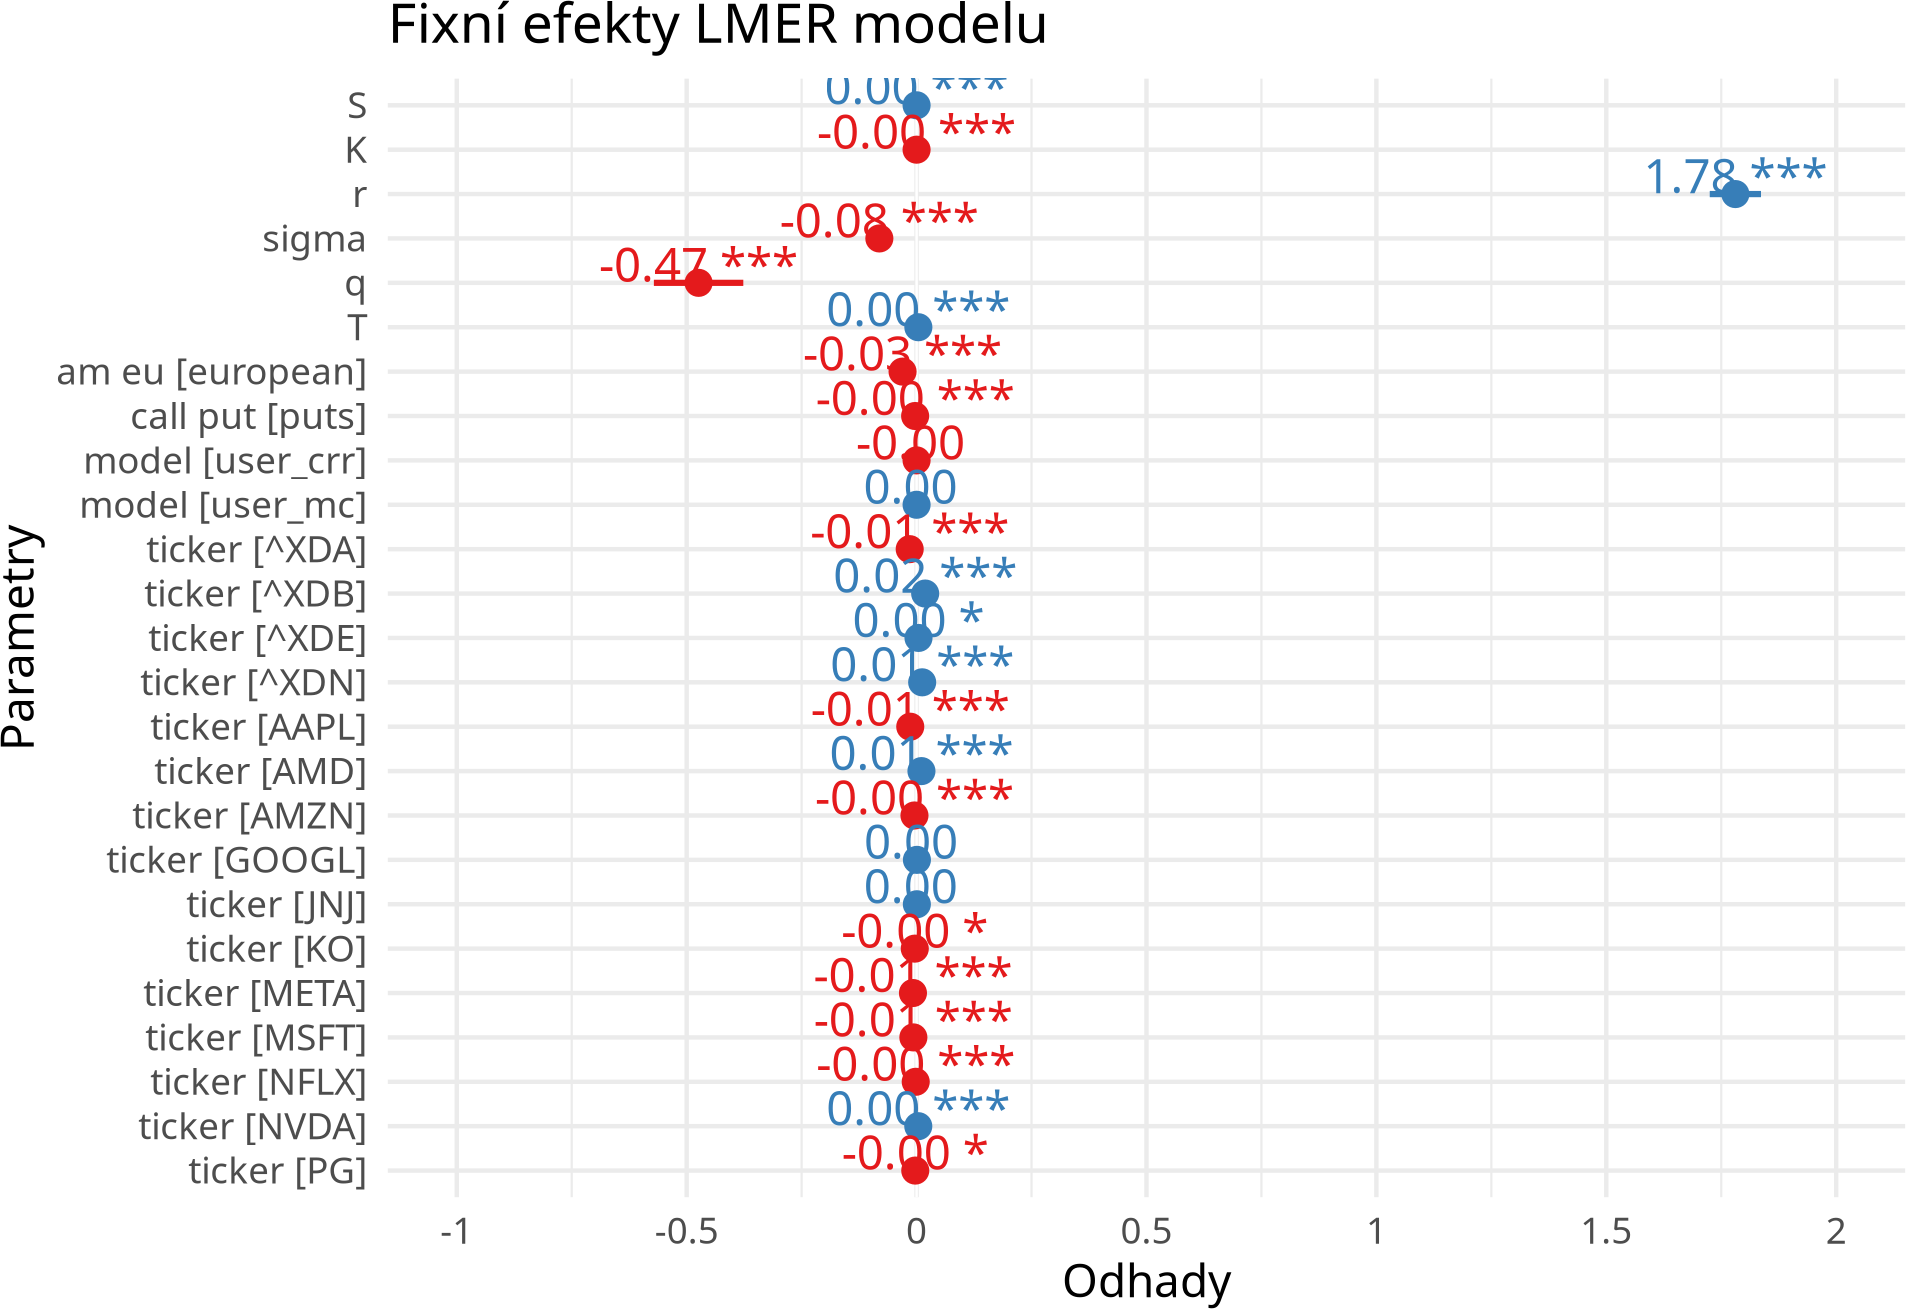
\includegraphics[keepaspectratio]{regression2_files/regression2_files/figure-latex/unnamed-chunk-9-1.png}}

\pandocbounded{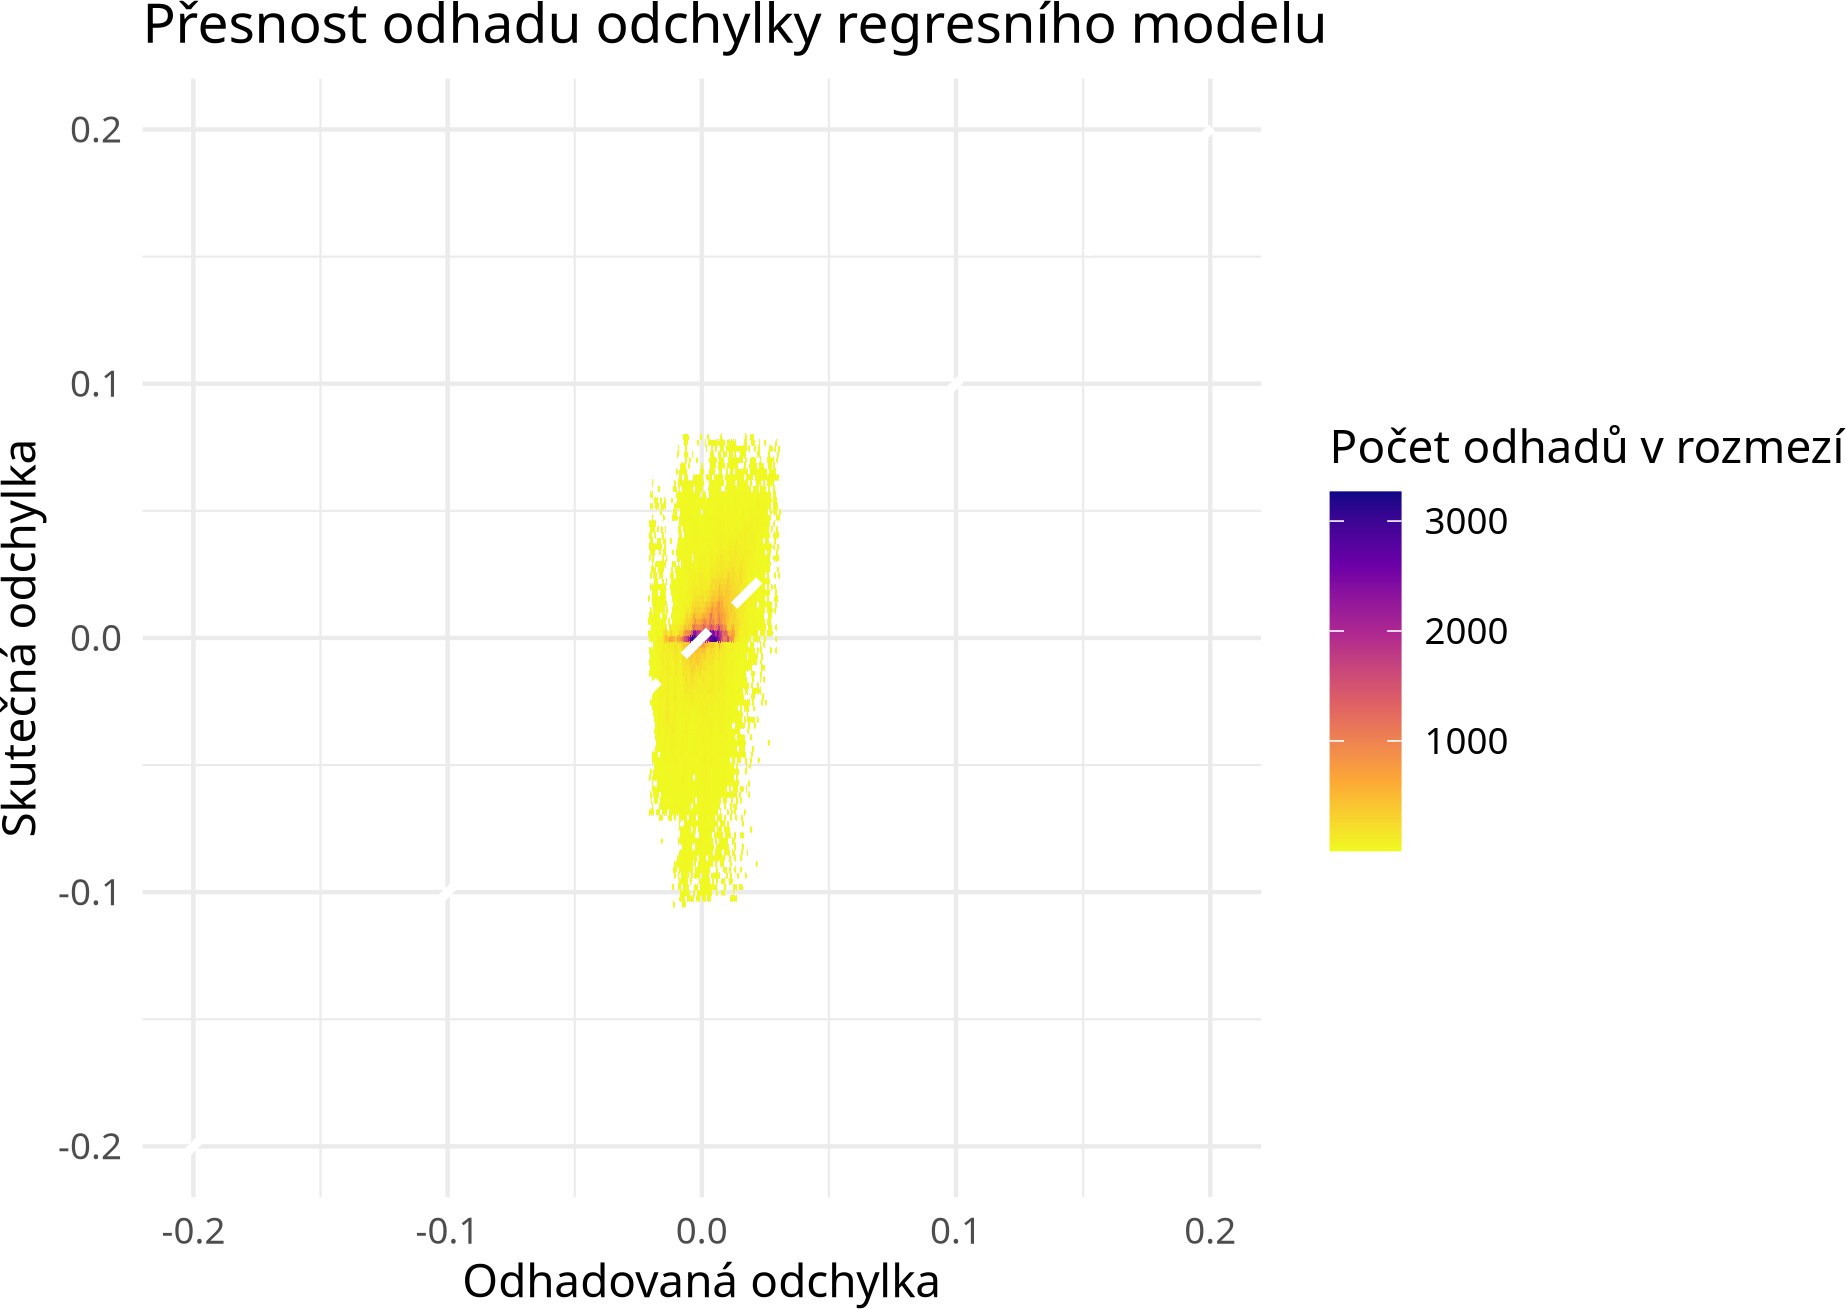
\includegraphics[keepaspectratio]{regression2_files/regression2_files/figure-latex/rmr_post_base_predict_fixed-1.png}}

\begin{Shaded}
\begin{Highlighting}[]
\FunctionTok{anova}\NormalTok{(rmr\_relative)}
\end{Highlighting}
\end{Shaded}

\begin{verbatim}
## Type III Analysis of Variance Table with Satterthwaite's method
##          Sum Sq Mean Sq NumDF  DenDF   F value Pr(>F)    
## S        0.1175 0.11746     1  83414  427.8228 <2e-16 ***
## K        0.7953 0.79528     1 329480 2896.5112 <2e-16 ***
## r        1.0765 1.07650     1 141352 3920.7494 <2e-16 ***
## sigma    1.1409 1.14089     1  59322 4155.2666 <2e-16 ***
## q        0.0251 0.02507     1 329356   91.2919 <2e-16 ***
## T        2.4051 2.40508     1 329399 8759.6239 <2e-16 ***
## am_eu    0.1139 0.11388     1  47677  414.7580 <2e-16 ***
## call_put 0.7486 0.74858     1 329483 2726.4416 <2e-16 ***
## model    0.0000 0.00002     2 329483    0.0592 0.9425    
## ticker   4.6973 0.31315    15 262975 1140.5449 <2e-16 ***
## ---
## Signif. codes:  0 '***' 0.001 '**' 0.01 '*' 0.05 '.' 0.1 ' ' 1
\end{verbatim}

\begin{Shaded}
\begin{Highlighting}[]
\FunctionTok{ranef}\NormalTok{(rmr\_relative)}
\end{Highlighting}
\end{Shaded}

\begin{verbatim}
## $snapshot_month
##      (Intercept)
## 01 -7.129052e-04
## 02  9.922789e-04
## 03 -5.833745e-05
## 05 -2.210362e-04
## 
## with conditional variances for "snapshot_month"
\end{verbatim}

\subsection{LMER model - náhodný
ticker}\label{lmer-model---nuxe1hodnuxfd-ticker}

Mnohem lepší \(R^2\), stále malé. Nevýznamný poměr \(S/K\) a styl
využití opce (a model).

\begin{Shaded}
\begin{Highlighting}[]
\NormalTok{subset\_args }\OtherTok{\textless{}{-}} \FunctionTok{c}\NormalTok{(}
  \CommentTok{\#"S",}
  \StringTok{"moneyness"}\NormalTok{,}
  \StringTok{"K"}\NormalTok{,}
  \StringTok{"r"}\NormalTok{,}
  \StringTok{"sigma"}\NormalTok{,}
  \StringTok{"q"}\NormalTok{,}
  \StringTok{"T"}\NormalTok{,}
  \StringTok{"am\_eu"}\NormalTok{,}
  \StringTok{"call\_put"}\NormalTok{,}
  \StringTok{"model"}
  \CommentTok{\#"ticker"}
\NormalTok{)}
\NormalTok{interactions }\OtherTok{\textless{}{-}} \FunctionTok{c}\NormalTok{(}
  \StringTok{"(1 | ticker)"}\NormalTok{,}
  \StringTok{"(1 | snapshot\_month)"}
\NormalTok{)}

\NormalTok{rhs }\OtherTok{\textless{}{-}} \FunctionTok{paste}\NormalTok{(}\FunctionTok{c}\NormalTok{(subset\_args, interactions), }\AttributeTok{collapse =} \StringTok{" + "}\NormalTok{)}
\NormalTok{formula }\OtherTok{\textless{}{-}} \FunctionTok{as.formula}\NormalTok{(}\FunctionTok{paste}\NormalTok{(}\StringTok{"pricing\_error \textasciitilde{} "}\NormalTok{, rhs))}

\NormalTok{rmr\_relative }\OtherTok{\textless{}{-}} \FunctionTok{lmer}\NormalTok{(formula, }\AttributeTok{data =}\NormalTok{ train\_data\_rel)}
\end{Highlighting}
\end{Shaded}

\begin{verbatim}
## Warning: Some predictor variables are on very different scales: consider rescaling. 
## You may also use (g)lmerControl(autoscale = TRUE) to improve numerical stability.
## Warning: Some predictor variables are on very different scales: consider rescaling. 
## You may also use (g)lmerControl(autoscale = TRUE) to improve numerical stability.
\end{verbatim}

\begin{Shaded}
\begin{Highlighting}[]
\FunctionTok{summary}\NormalTok{(rmr\_relative)}
\end{Highlighting}
\end{Shaded}

\begin{verbatim}
## Linear mixed model fit by REML. t-tests use Satterthwaite's method [
## lmerModLmerTest]
## Formula: formula
##    Data: train_data_rel
## 
## REML criterion at convergence: -1766277
## 
## Scaled residuals: 
##     Min      1Q  Median      3Q     Max 
## -7.0098 -0.3318  0.0604  0.4445  5.1863 
## 
## Random effects:
##  Groups         Name        Variance  Std.Dev. 
##  ticker         (Intercept) 9.816e-05 0.0099075
##  snapshot_month (Intercept) 6.710e-07 0.0008192
##  Residual                   2.749e-04 0.0165805
## Number of obs: 329512, groups:  ticker, 17; snapshot_month, 4
## 
## Fixed effects:
##                 Estimate Std. Error         df t value Pr(>|t|)    
## (Intercept)   -3.043e-02  3.140e-03  2.101e+01  -9.691 3.33e-09 ***
## moneyness      9.876e-05  3.307e-05  3.285e+05   2.987  0.00282 ** 
## K             -6.864e-06  1.596e-07  3.179e+05 -43.008  < 2e-16 ***
## r              1.765e+00  2.846e-02  1.847e+05  62.027  < 2e-16 ***
## sigma         -7.654e-02  1.238e-03  1.113e+05 -61.801  < 2e-16 ***
## q             -5.477e-01  4.840e-02  7.261e+03 -11.316  < 2e-16 ***
## T              3.863e-03  4.169e-05  3.295e+05  92.647  < 2e-16 ***
## am_eueuropean -1.984e-02  5.334e-03  1.519e+01  -3.719  0.00202 ** 
## call_putputs  -3.112e-03  6.034e-05  3.295e+05 -51.571  < 2e-16 ***
## modeluser_crr -9.530e-06  7.075e-05  3.295e+05  -0.135  0.89285    
## modeluser_mc   1.392e-05  7.075e-05  3.295e+05   0.197  0.84407    
## ---
## Signif. codes:  0 '***' 0.001 '**' 0.01 '*' 0.05 '.' 0.1 ' ' 1
## 
## Correlation of Fixed Effects:
##             (Intr) mnynss K      r      sigma  q      T      am_rpn cll_pt
## moneyness   -0.020                                                        
## K           -0.016  0.500                                                 
## r           -0.334  0.019  0.007                                          
## sigma       -0.138 -0.057 -0.069  0.002                                   
## q           -0.143  0.011  0.005 -0.026  0.048                            
## T           -0.058 -0.100 -0.075  0.157 -0.007  0.001                     
## am_eueuropn -0.508 -0.005 -0.012 -0.002  0.057  0.088  0.003              
## call_putpts -0.006 -0.038  0.211 -0.011 -0.014  0.000 -0.018 -0.002       
## modelsr_crr -0.011  0.000  0.000  0.000  0.000 -0.001  0.000  0.000  0.000
## modelusr_mc -0.011 -0.001 -0.001  0.000  0.001 -0.001  0.000  0.000  0.001
##             mdlsr_c
## moneyness          
## K                  
## r                  
## sigma              
## q                  
## T                  
## am_eueuropn        
## call_putpts        
## modelsr_crr        
## modelusr_mc  0.500 
## fit warnings:
## Some predictor variables are on very different scales: consider rescaling. 
## You may also use (g)lmerControl(autoscale = TRUE) to improve numerical stability.
\end{verbatim}

\begin{Shaded}
\begin{Highlighting}[]
\FunctionTok{r2}\NormalTok{(rmr\_relative)}
\end{Highlighting}
\end{Shaded}

\begin{verbatim}
## Warning: Can't compute random effect variances. Some variance components equal
##   zero. Your model may suffer from singularity (see `?lme4::isSingular`
##   and `?performance::check_singularity`).
##   Decrease the `tolerance` level to force the calculation of random effect
##   variances, or impose priors on your random effects parameters (using
##   packages like `brms` or `glmmTMB`).
\end{verbatim}

\begin{verbatim}
## Random effect variances not available. Returned R2 does not account for random effects.
\end{verbatim}

\begin{verbatim}
## # R2 for Mixed Models
## 
##   Conditional R2: NA
##      Marginal R2: 0.321
\end{verbatim}

\pandocbounded{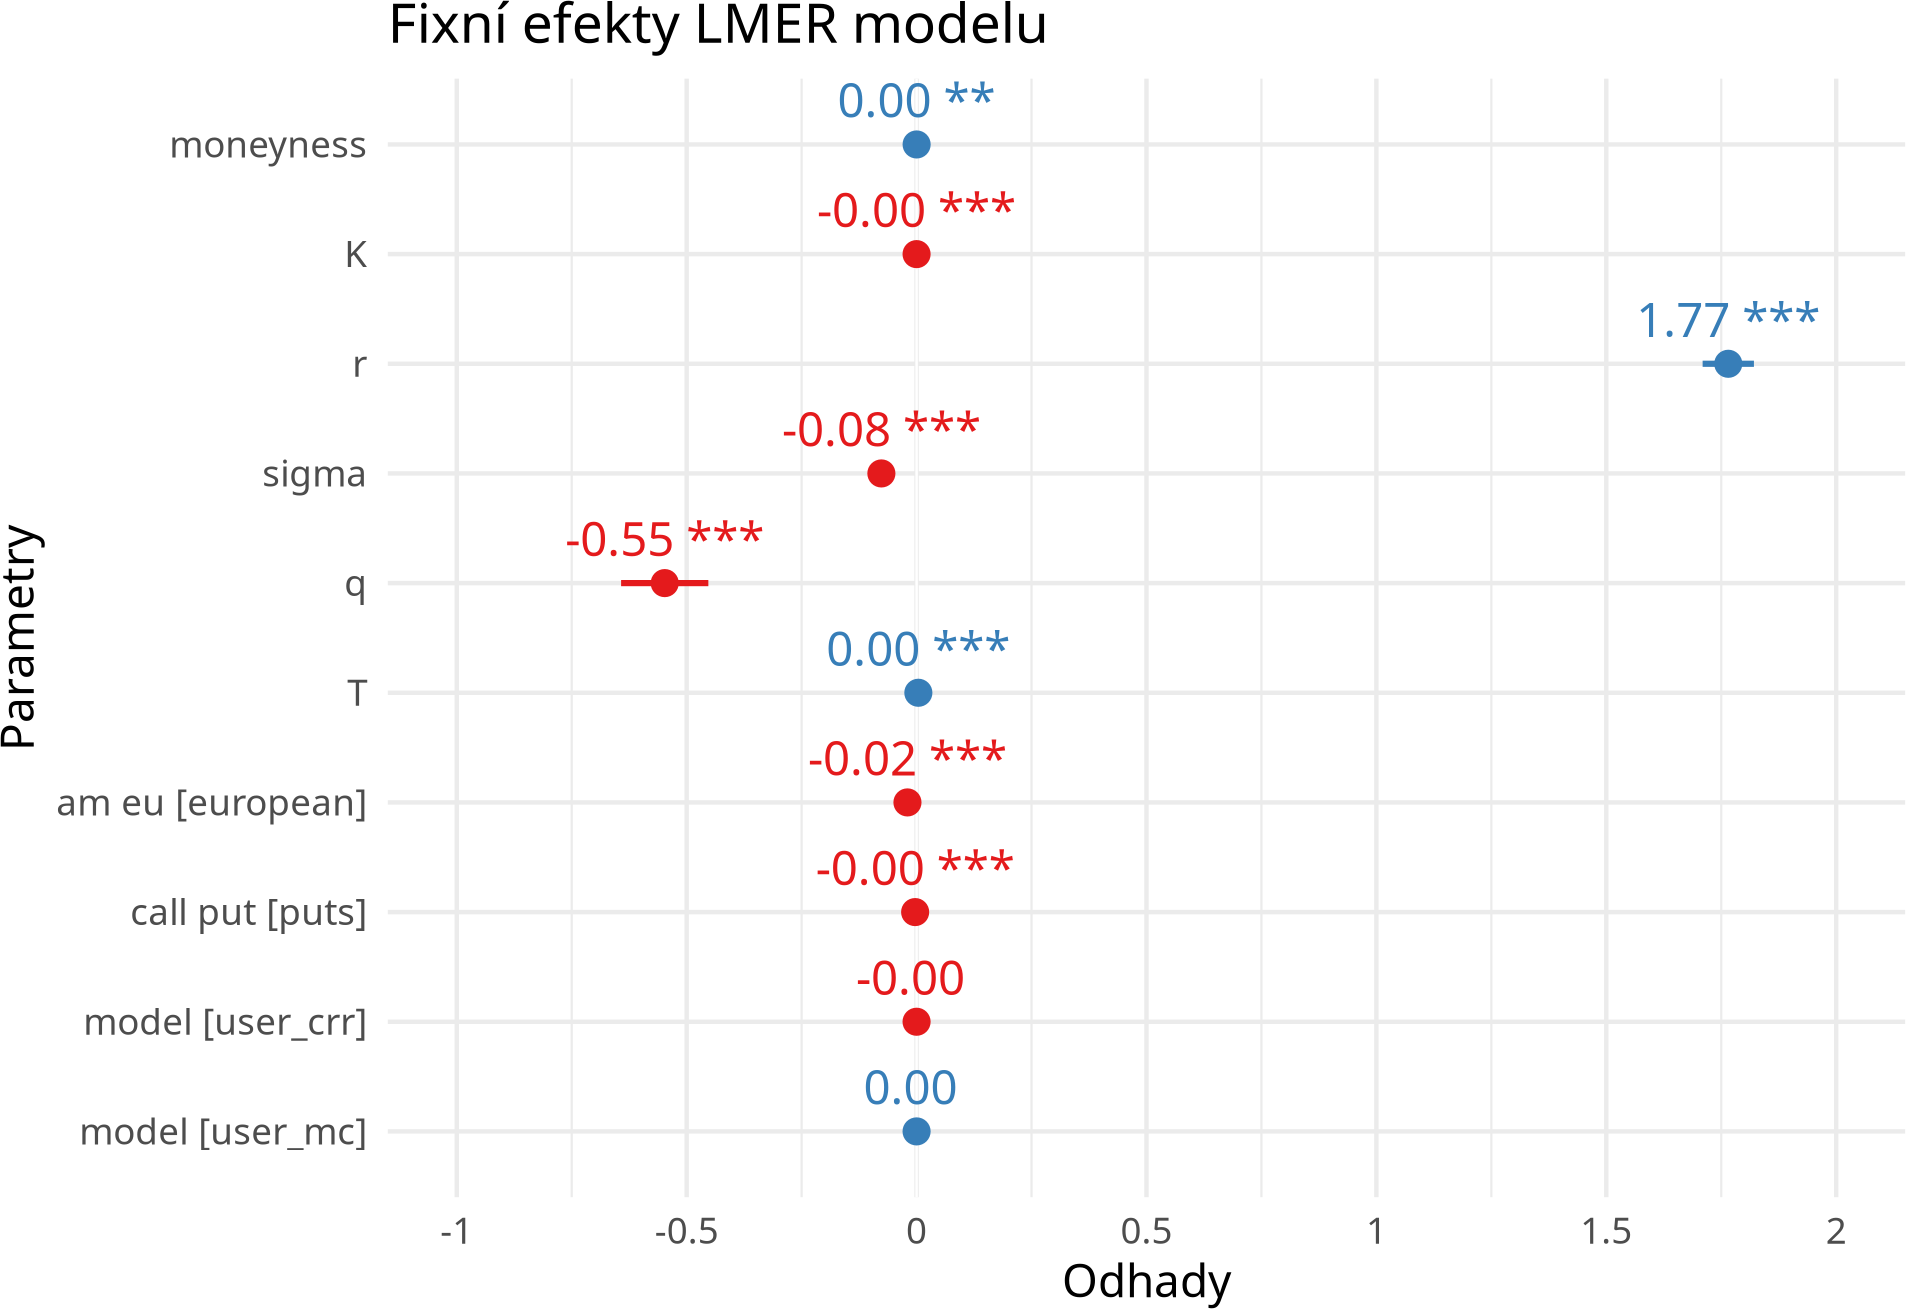
\includegraphics[keepaspectratio]{regression2_files/regression2_files/figure-latex/unnamed-chunk-14-1.png}}

\pandocbounded{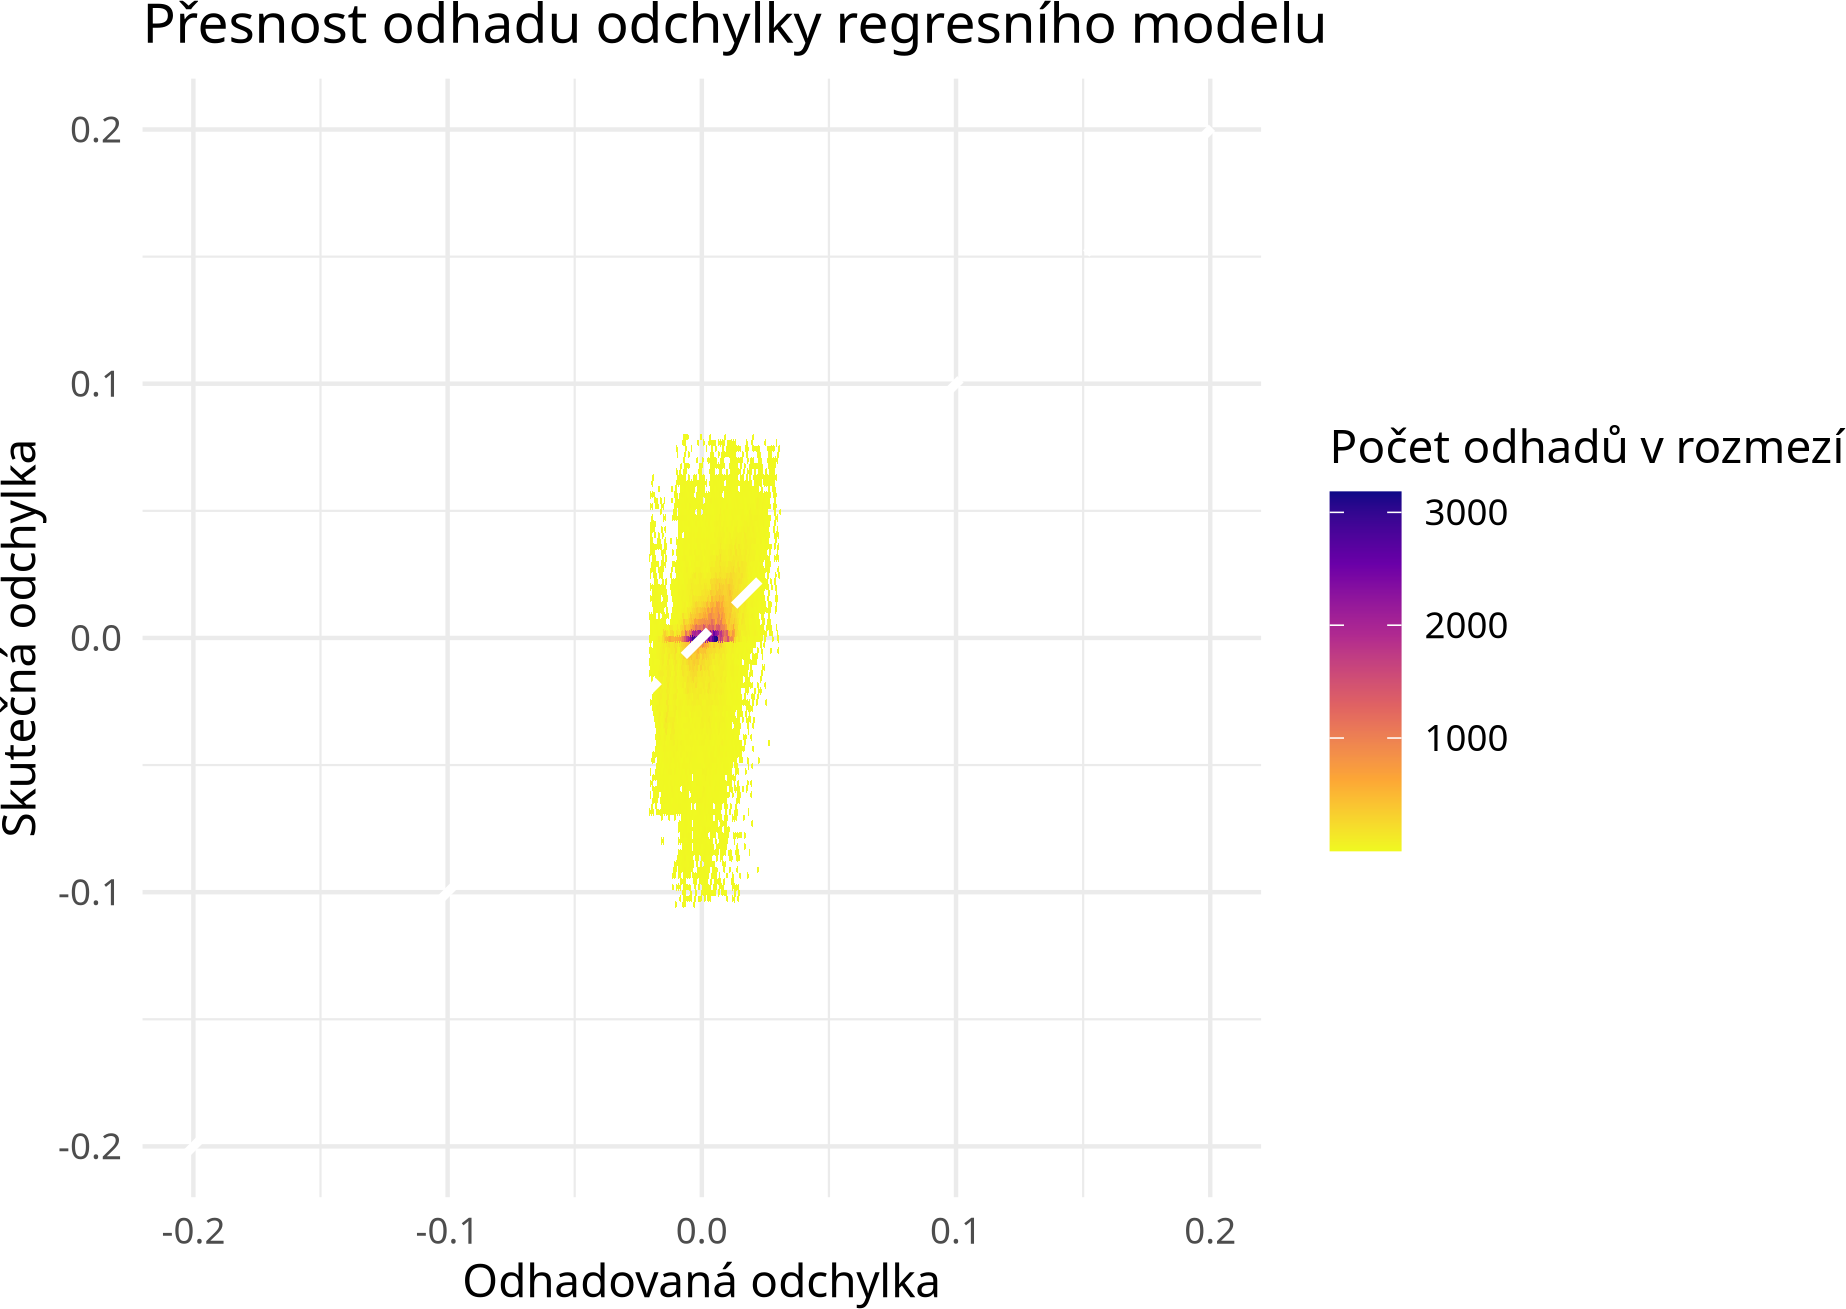
\includegraphics[keepaspectratio]{regression2_files/regression2_files/figure-latex/rmr_post_base_predict_rand-1.png}}

\begin{Shaded}
\begin{Highlighting}[]
\FunctionTok{anova}\NormalTok{(rmr\_relative)}
\end{Highlighting}
\end{Shaded}

\begin{verbatim}
## Type III Analysis of Variance Table with Satterthwaite's method
##            Sum Sq Mean Sq NumDF  DenDF   F value    Pr(>F)    
## moneyness 0.00245 0.00245     1 328514    8.9215  0.002818 ** 
## K         0.50850 0.50850     1 317863 1849.6632 < 2.2e-16 ***
## r         1.05768 1.05768     1 184707 3847.3058 < 2.2e-16 ***
## sigma     1.04999 1.04999     1 111346 3819.3525 < 2.2e-16 ***
## q         0.03520 0.03520     1   7261  128.0488 < 2.2e-16 ***
## T         2.35972 2.35972     1 329452 8583.5268 < 2.2e-16 ***
## am_eu     0.00380 0.00380     1     15   13.8308  0.002017 ** 
## call_put  0.73116 0.73116     1 329485 2659.6153 < 2.2e-16 ***
## model     0.00003 0.00002     2 329483    0.0555  0.945970    
## ---
## Signif. codes:  0 '***' 0.001 '**' 0.01 '*' 0.05 '.' 0.1 ' ' 1
\end{verbatim}

\begin{Shaded}
\begin{Highlighting}[]
\FunctionTok{ranef}\NormalTok{(rmr\_relative)}
\end{Highlighting}
\end{Shaded}

\begin{verbatim}
## $ticker
##         (Intercept)
## ^RUT   0.0198248629
## ^XDA  -0.0246242852
## ^XDB   0.0088074687
## ^XDE  -0.0055644258
## ^XDN   0.0015563796
## AAPL  -0.0117662628
## AMD    0.0110811235
## AMZN  -0.0036266622
## GOOGL  0.0033001023
## JNJ    0.0047768113
## KO    -0.0017662644
## META  -0.0023118431
## MSFT  -0.0028877790
## NFLX  -0.0025451289
## NVDA   0.0038170048
## PG    -0.0001604142
## TSLA   0.0020893125
## 
## $snapshot_month
##      (Intercept)
## 01 -0.0006664638
## 02  0.0008346210
## 03 -0.0007334943
## 05  0.0005653371
## 
## with conditional variances for "ticker" "snapshot_month"
\end{verbatim}

\subsection{LMER model - náhodný ticker (fixní efekt měsíce
sběru)}\label{lmer-model---nuxe1hodnuxfd-ticker-fixnuxed-efekt-mux11bsuxedce-sbux11bru}

Stejné významnosti jako model s náhodným efektem měsíce, menší mezní
\(R^2\) než u předchozího modelu, podmíněné \(R^2\) je větší než mezní
\(R^2\) předchozího modelu.

\begin{Shaded}
\begin{Highlighting}[]
\NormalTok{subset\_args }\OtherTok{\textless{}{-}} \FunctionTok{c}\NormalTok{(}
  \CommentTok{\#"S",}
  \StringTok{"moneyness"}\NormalTok{,}
  \StringTok{"K"}\NormalTok{,}
  \StringTok{"r"}\NormalTok{,}
  \StringTok{"sigma"}\NormalTok{,}
  \StringTok{"q"}\NormalTok{,}
  \StringTok{"T"}\NormalTok{,}
  \StringTok{"am\_eu"}\NormalTok{,}
  \StringTok{"call\_put"}\NormalTok{,}
  \StringTok{"snapshot\_month"}\NormalTok{,}
  \StringTok{"model"}
  \CommentTok{\#"ticker"}
\NormalTok{)}
\NormalTok{interactions }\OtherTok{\textless{}{-}} \FunctionTok{c}\NormalTok{(}
  \StringTok{"(1 | ticker)"}
  \CommentTok{\#"(1 | snapshot\_month)"}
\NormalTok{)}

\NormalTok{rhs }\OtherTok{\textless{}{-}} \FunctionTok{paste}\NormalTok{(}\FunctionTok{c}\NormalTok{(subset\_args, interactions), }\AttributeTok{collapse =} \StringTok{" + "}\NormalTok{)}
\NormalTok{formula }\OtherTok{\textless{}{-}} \FunctionTok{as.formula}\NormalTok{(}\FunctionTok{paste}\NormalTok{(}\StringTok{"pricing\_error \textasciitilde{} "}\NormalTok{, rhs))}

\NormalTok{rmr\_relative }\OtherTok{\textless{}{-}} \FunctionTok{lmer}\NormalTok{(formula, }\AttributeTok{data =}\NormalTok{ train\_data\_rel)}
\end{Highlighting}
\end{Shaded}

\begin{verbatim}
## Warning: Some predictor variables are on very different scales: consider rescaling. 
## You may also use (g)lmerControl(autoscale = TRUE) to improve numerical stability.
## Warning: Some predictor variables are on very different scales: consider rescaling. 
## You may also use (g)lmerControl(autoscale = TRUE) to improve numerical stability.
\end{verbatim}

\begin{Shaded}
\begin{Highlighting}[]
\FunctionTok{summary}\NormalTok{(rmr\_relative)}
\end{Highlighting}
\end{Shaded}

\begin{verbatim}
## Linear mixed model fit by REML. t-tests use Satterthwaite's method [
## lmerModLmerTest]
## Formula: formula
##    Data: train_data_rel
## 
## REML criterion at convergence: -1766244
## 
## Scaled residuals: 
##     Min      1Q  Median      3Q     Max 
## -7.0101 -0.3318  0.0604  0.4445  5.1860 
## 
## Random effects:
##  Groups   Name        Variance  Std.Dev.
##  ticker   (Intercept) 9.812e-05 0.009906
##  Residual             2.749e-04 0.016581
## Number of obs: 329512, groups:  ticker, 17
## 
## Fixed effects:
##                    Estimate Std. Error         df t value Pr(>|t|)    
## (Intercept)      -3.114e-02  3.112e-03  2.036e+01 -10.006 2.62e-09 ***
## moneyness         9.848e-05  3.307e-05  3.290e+05   2.978  0.00290 ** 
## K                -6.866e-06  1.596e-07  3.190e+05 -43.015  < 2e-16 ***
## r                 1.766e+00  2.850e-02  3.295e+05  61.965  < 2e-16 ***
## sigma            -7.649e-02  1.241e-03  2.776e+05 -61.636  < 2e-16 ***
## q                -5.473e-01  4.840e-02  7.259e+03 -11.306  < 2e-16 ***
## T                 3.863e-03  4.169e-05  3.295e+05  92.653  < 2e-16 ***
## am_eueuropean    -1.982e-02  5.333e-03  1.520e+01  -3.717  0.00203 ** 
## call_putputs     -3.112e-03  6.034e-05  3.295e+05 -51.574  < 2e-16 ***
## snapshot_month02  1.509e-03  8.419e-05  3.291e+05  17.925  < 2e-16 ***
## snapshot_month03 -6.770e-05  8.925e-05  3.295e+05  -0.759  0.44814    
## snapshot_month05  1.240e-03  1.090e-04  3.262e+05  11.373  < 2e-16 ***
## modeluser_crr    -9.542e-06  7.075e-05  3.295e+05  -0.135  0.89272    
## modeluser_mc      1.391e-05  7.075e-05  3.295e+05   0.197  0.84410    
## ---
## Signif. codes:  0 '***' 0.001 '**' 0.01 '*' 0.05 '.' 0.1 ' ' 1
\end{verbatim}

\begin{verbatim}
## 
## Correlation matrix not shown by default, as p = 14 > 12.
## Use print(x, correlation=TRUE)  or
##     vcov(x)        if you need it
\end{verbatim}

\begin{verbatim}
## fit warnings:
## Some predictor variables are on very different scales: consider rescaling. 
## You may also use (g)lmerControl(autoscale = TRUE) to improve numerical stability.
\end{verbatim}

\begin{Shaded}
\begin{Highlighting}[]
\FunctionTok{r2}\NormalTok{(rmr\_relative)}
\end{Highlighting}
\end{Shaded}

\begin{verbatim}
## # R2 for Mixed Models
## 
##   Conditional R2: 0.454
##      Marginal R2: 0.259
\end{verbatim}

\pandocbounded{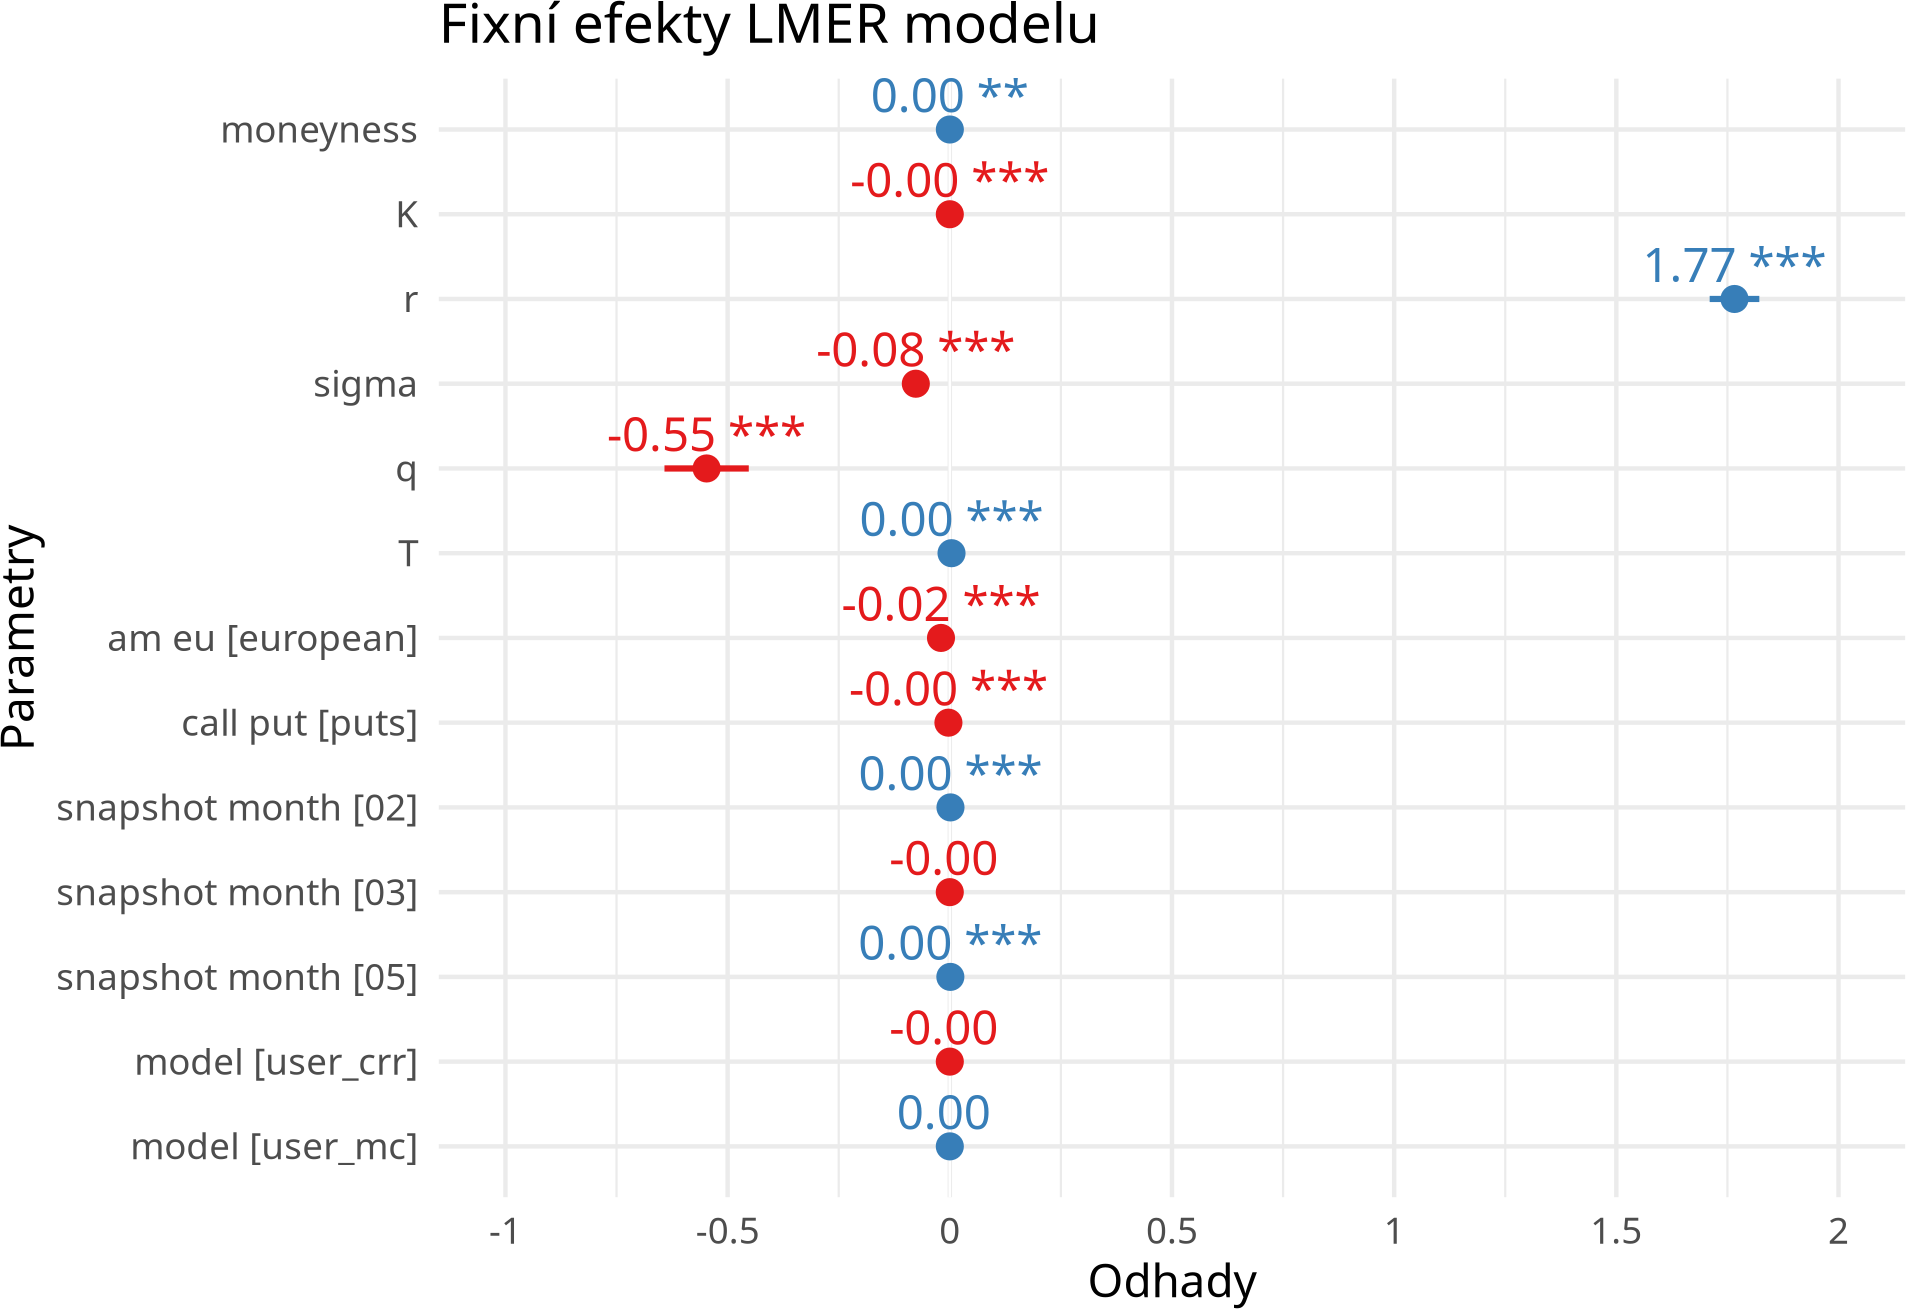
\includegraphics[keepaspectratio]{regression2_files/regression2_files/figure-latex/unnamed-chunk-19-1.png}}

\pandocbounded{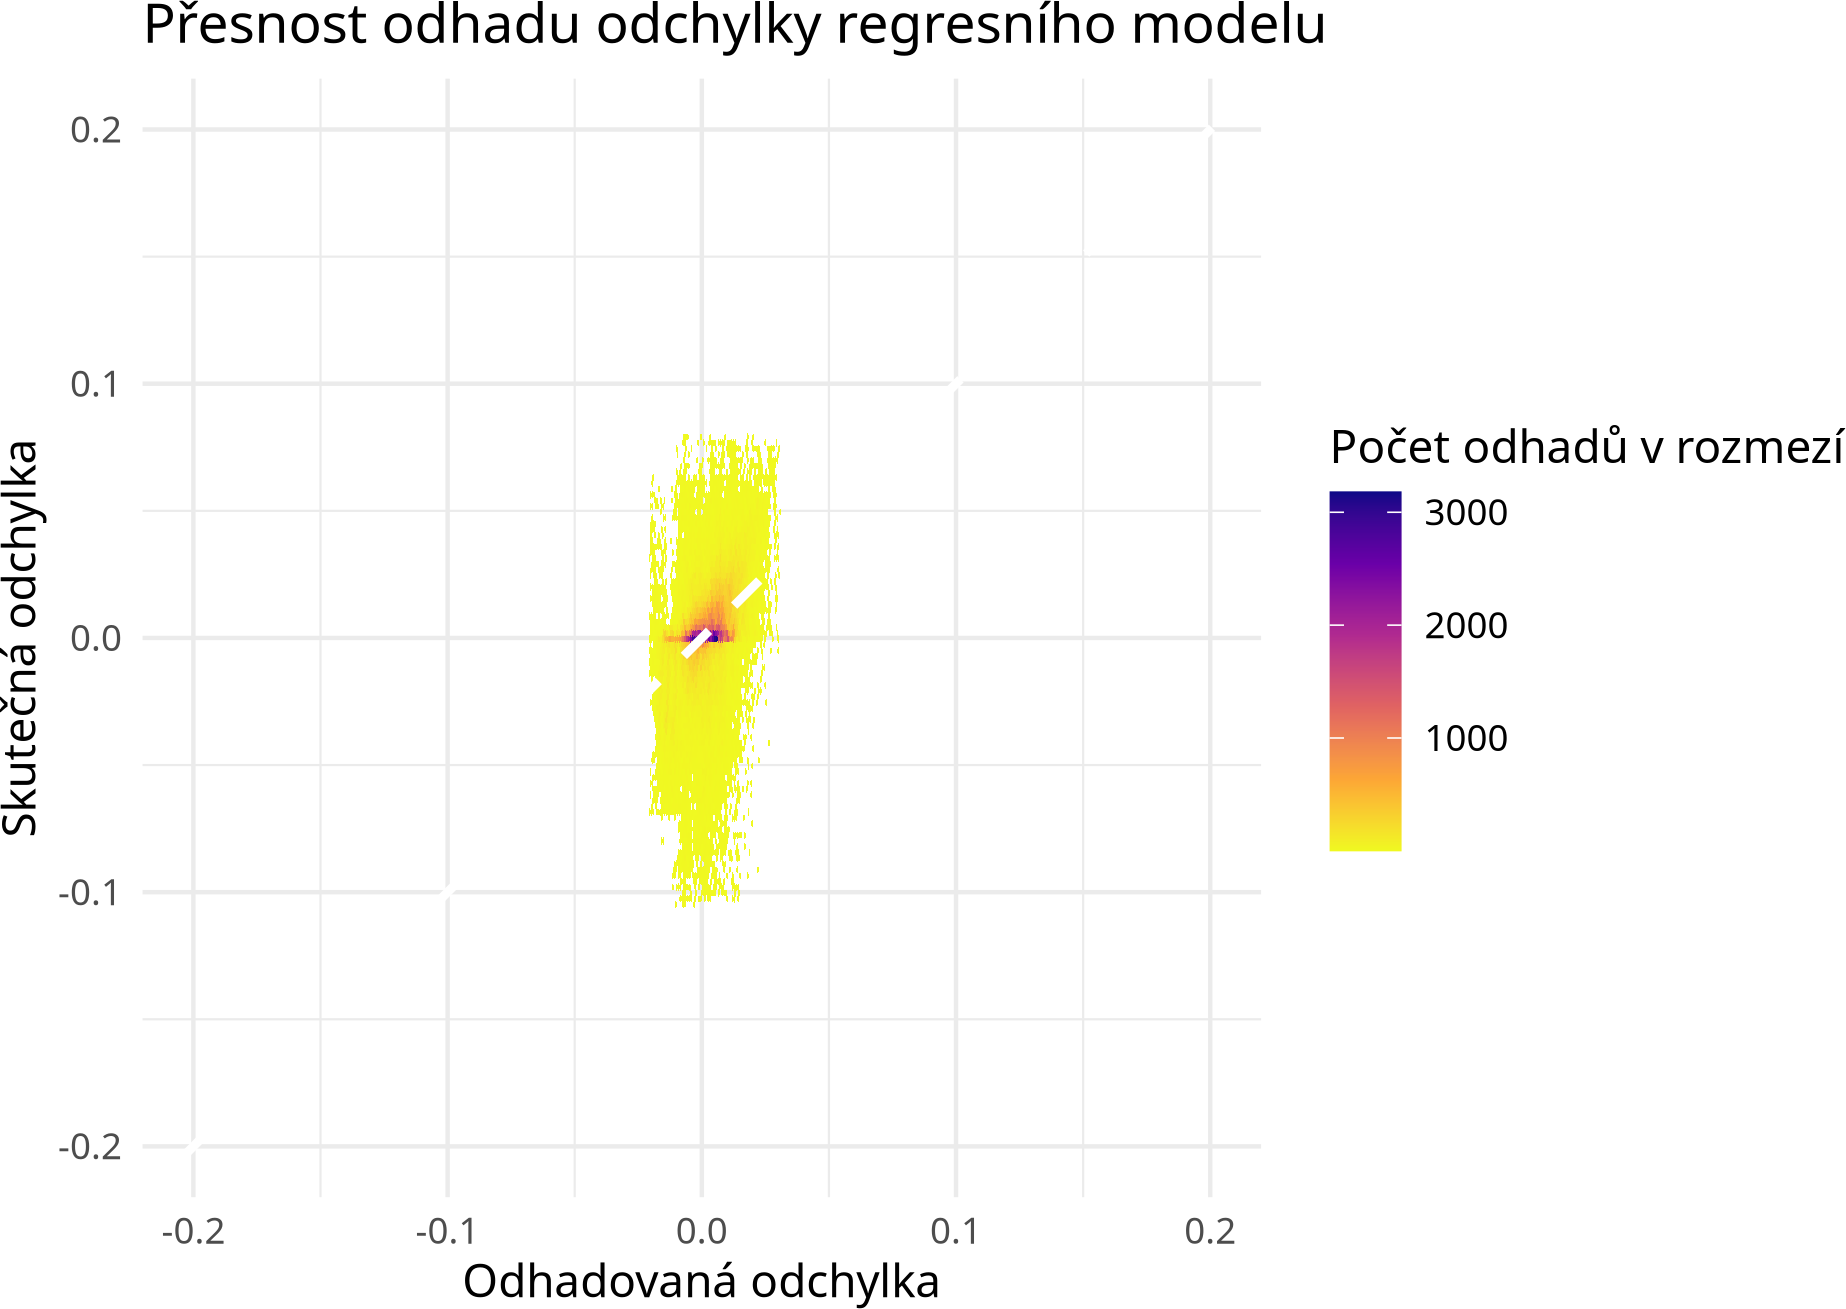
\includegraphics[keepaspectratio]{regression2_files/regression2_files/figure-latex/rmr_post_base_predict_rand2-1.png}}

\begin{Shaded}
\begin{Highlighting}[]
\FunctionTok{anova}\NormalTok{(rmr\_relative)}
\end{Highlighting}
\end{Shaded}

\begin{verbatim}
## Type III Analysis of Variance Table with Satterthwaite's method
##                 Sum Sq Mean Sq NumDF  DenDF   F value    Pr(>F)    
## moneyness      0.00244 0.00244     1 328987    8.8704  0.002899 ** 
## K              0.50867 0.50867     1 319024 1850.2913 < 2.2e-16 ***
## r              1.05558 1.05558     1 329496 3839.6935 < 2.2e-16 ***
## sigma          1.04439 1.04439     1 277623 3798.9940 < 2.2e-16 ***
## q              0.03514 0.03514     1   7259  127.8279 < 2.2e-16 ***
## T              2.36000 2.36000     1 329490 8584.5360 < 2.2e-16 ***
## am_eu          0.00380 0.00380     1     15   13.8132  0.002026 ** 
## call_put       0.73122 0.73122     1 329483 2659.8382 < 2.2e-16 ***
## snapshot_month 0.14439 0.04813     3 327415  175.0688 < 2.2e-16 ***
## model          0.00003 0.00002     2 329483    0.0556  0.945932    
## ---
## Signif. codes:  0 '***' 0.001 '**' 0.01 '*' 0.05 '.' 0.1 ' ' 1
\end{verbatim}

\begin{Shaded}
\begin{Highlighting}[]
\FunctionTok{ranef}\NormalTok{(rmr\_relative)}
\end{Highlighting}
\end{Shaded}

\begin{verbatim}
## $ticker
##         (Intercept)
## ^RUT   0.0198232763
## ^XDA  -0.0246245864
## ^XDB   0.0088089399
## ^XDE  -0.0055634411
## ^XDN   0.0015558108
## AAPL  -0.0117619301
## AMD    0.0110707091
## AMZN  -0.0036223174
## GOOGL  0.0033037797
## JNJ    0.0047728753
## KO    -0.0017680271
## META  -0.0023104190
## MSFT  -0.0028828390
## NFLX  -0.0025405844
## NVDA   0.0038173705
## PG    -0.0001614436
## TSLA   0.0020828256
## 
## with conditional variances for "ticker"
\end{verbatim}

\subsection{LMER model - náhodný ticker (žádný efekt
měsíce)}\label{lmer-model---nuxe1hodnuxfd-ticker-ux17euxe1dnuxfd-efekt-mux11bsuxedce}

Všechny parametry statisticky významné, lepší \(R^2\) než u předchozího
modelu. Mezní \(R^2\) stále horší než u modelu s náhodným efektem
měsíce.

\begin{Shaded}
\begin{Highlighting}[]
\NormalTok{subset\_args }\OtherTok{\textless{}{-}} \FunctionTok{c}\NormalTok{(}
  \CommentTok{\#"S",}
  \StringTok{"moneyness"}\NormalTok{,}
  \StringTok{"K"}\NormalTok{,}
  \StringTok{"r"}\NormalTok{,}
  \StringTok{"sigma"}\NormalTok{,}
  \StringTok{"q"}\NormalTok{,}
  \StringTok{"T"}\NormalTok{,}
  \StringTok{"am\_eu"}\NormalTok{,}
  \StringTok{"call\_put"}\NormalTok{,}
  \StringTok{"model"}
  \CommentTok{\#"ticker"}
\NormalTok{)}
\NormalTok{interactions }\OtherTok{\textless{}{-}} \FunctionTok{c}\NormalTok{(}
  \StringTok{"(1 | ticker)"}
  \CommentTok{\#"(1 | snapshot\_month)"}
\NormalTok{)}

\NormalTok{rhs }\OtherTok{\textless{}{-}} \FunctionTok{paste}\NormalTok{(}\FunctionTok{c}\NormalTok{(subset\_args, interactions), }\AttributeTok{collapse =} \StringTok{" + "}\NormalTok{)}
\NormalTok{formula }\OtherTok{\textless{}{-}} \FunctionTok{as.formula}\NormalTok{(}\FunctionTok{paste}\NormalTok{(}\StringTok{"pricing\_error \textasciitilde{} "}\NormalTok{, rhs))}

\NormalTok{rmr\_relative }\OtherTok{\textless{}{-}} \FunctionTok{lmer}\NormalTok{(formula, }\AttributeTok{data =}\NormalTok{ train\_data\_rel)}
\end{Highlighting}
\end{Shaded}

\begin{verbatim}
## Warning: Some predictor variables are on very different scales: consider rescaling. 
## You may also use (g)lmerControl(autoscale = TRUE) to improve numerical stability.
## Warning: Some predictor variables are on very different scales: consider rescaling. 
## You may also use (g)lmerControl(autoscale = TRUE) to improve numerical stability.
\end{verbatim}

\begin{Shaded}
\begin{Highlighting}[]
\FunctionTok{summary}\NormalTok{(rmr\_relative)}
\end{Highlighting}
\end{Shaded}

\begin{verbatim}
## Linear mixed model fit by REML. t-tests use Satterthwaite's method [
## lmerModLmerTest]
## Formula: formula
##    Data: train_data_rel
## 
## REML criterion at convergence: -1765770
## 
## Scaled residuals: 
##     Min      1Q  Median      3Q     Max 
## -6.9596 -0.3304  0.0579  0.4389  5.2279 
## 
## Random effects:
##  Groups   Name        Variance  Std.Dev.
##  ticker   (Intercept) 0.0001032 0.01016 
##  Residual             0.0002753 0.01659 
## Number of obs: 329512, groups:  ticker, 17
## 
## Fixed effects:
##                 Estimate Std. Error         df t value Pr(>|t|)    
## (Intercept)   -2.251e-02  3.146e-03  1.930e+01  -7.153 7.73e-07 ***
## moneyness      1.383e-04  3.284e-05  3.290e+05   4.210 2.55e-05 ***
## K             -6.594e-06  1.579e-07  3.188e+05 -41.759  < 2e-16 ***
## r              1.636e+00  2.416e-02  3.286e+05  67.724  < 2e-16 ***
## sigma         -8.373e-02  9.635e-04  3.072e+05 -86.906  < 2e-16 ***
## q             -6.303e-01  4.830e-02  7.947e+03 -13.050  < 2e-16 ***
## T              3.807e-03  4.160e-05  3.295e+05  91.520  < 2e-16 ***
## am_eueuropean -2.227e-02  5.463e-03  1.518e+01  -4.077 0.000969 ***
## call_putputs  -3.091e-03  6.037e-05  3.295e+05 -51.194  < 2e-16 ***
## modeluser_crr -7.615e-06  7.081e-05  3.295e+05  -0.108 0.914356    
## modeluser_mc   1.432e-05  7.081e-05  3.295e+05   0.202 0.839696    
## ---
## Signif. codes:  0 '***' 0.001 '**' 0.01 '*' 0.05 '.' 0.1 ' ' 1
## 
## Correlation of Fixed Effects:
##             (Intr) mnynss K      r      sigma  q      T      am_rpn cll_pt
## moneyness   -0.023                                                        
## K           -0.019  0.491                                                 
## r           -0.314  0.001 -0.023                                          
## sigma       -0.197  0.012  0.023  0.314                                   
## q           -0.139  0.013  0.009 -0.031  0.029                            
## T           -0.047 -0.100 -0.074  0.144  0.000 -0.001                     
## am_eueuropn -0.520 -0.001 -0.007  0.010  0.042  0.084  0.003              
## call_putpts -0.007 -0.041  0.210 -0.015 -0.001  0.001 -0.017 -0.002       
## modelsr_crr -0.011  0.000  0.000  0.000  0.001 -0.001  0.000  0.000  0.000
## modelusr_mc -0.011 -0.001 -0.001  0.000  0.002 -0.001  0.000  0.000  0.001
##             mdlsr_c
## moneyness          
## K                  
## r                  
## sigma              
## q                  
## T                  
## am_eueuropn        
## call_putpts        
## modelsr_crr        
## modelusr_mc  0.500 
## fit warnings:
## Some predictor variables are on very different scales: consider rescaling. 
## You may also use (g)lmerControl(autoscale = TRUE) to improve numerical stability.
\end{verbatim}

\begin{Shaded}
\begin{Highlighting}[]
\FunctionTok{r2}\NormalTok{(rmr\_relative)}
\end{Highlighting}
\end{Shaded}

\begin{verbatim}
## # R2 for Mixed Models
## 
##   Conditional R2: 0.471
##      Marginal R2: 0.273
\end{verbatim}

\pandocbounded{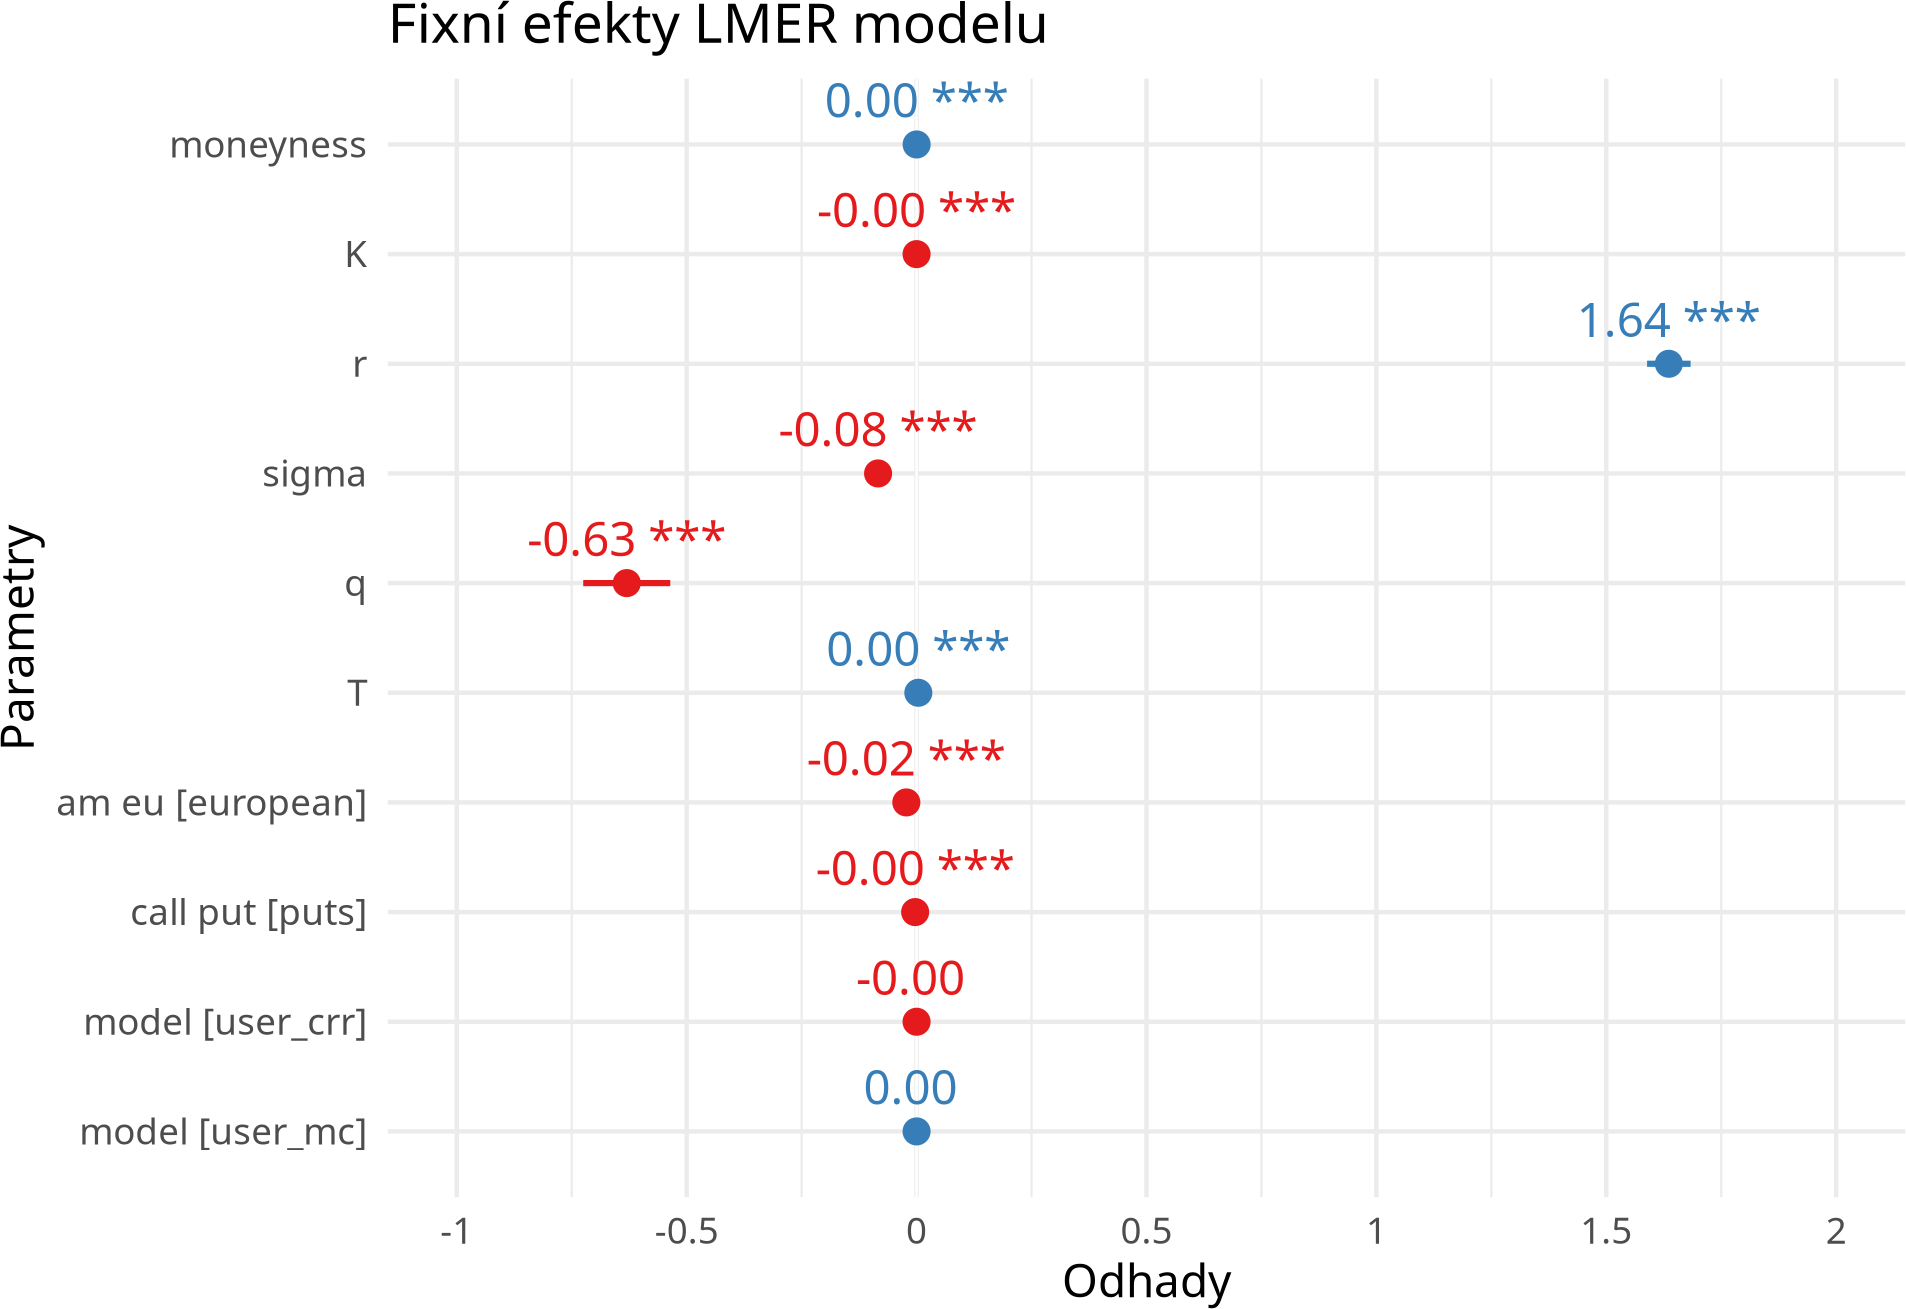
\includegraphics[keepaspectratio]{regression2_files/regression2_files/figure-latex/unnamed-chunk-24-1.png}}

\pandocbounded{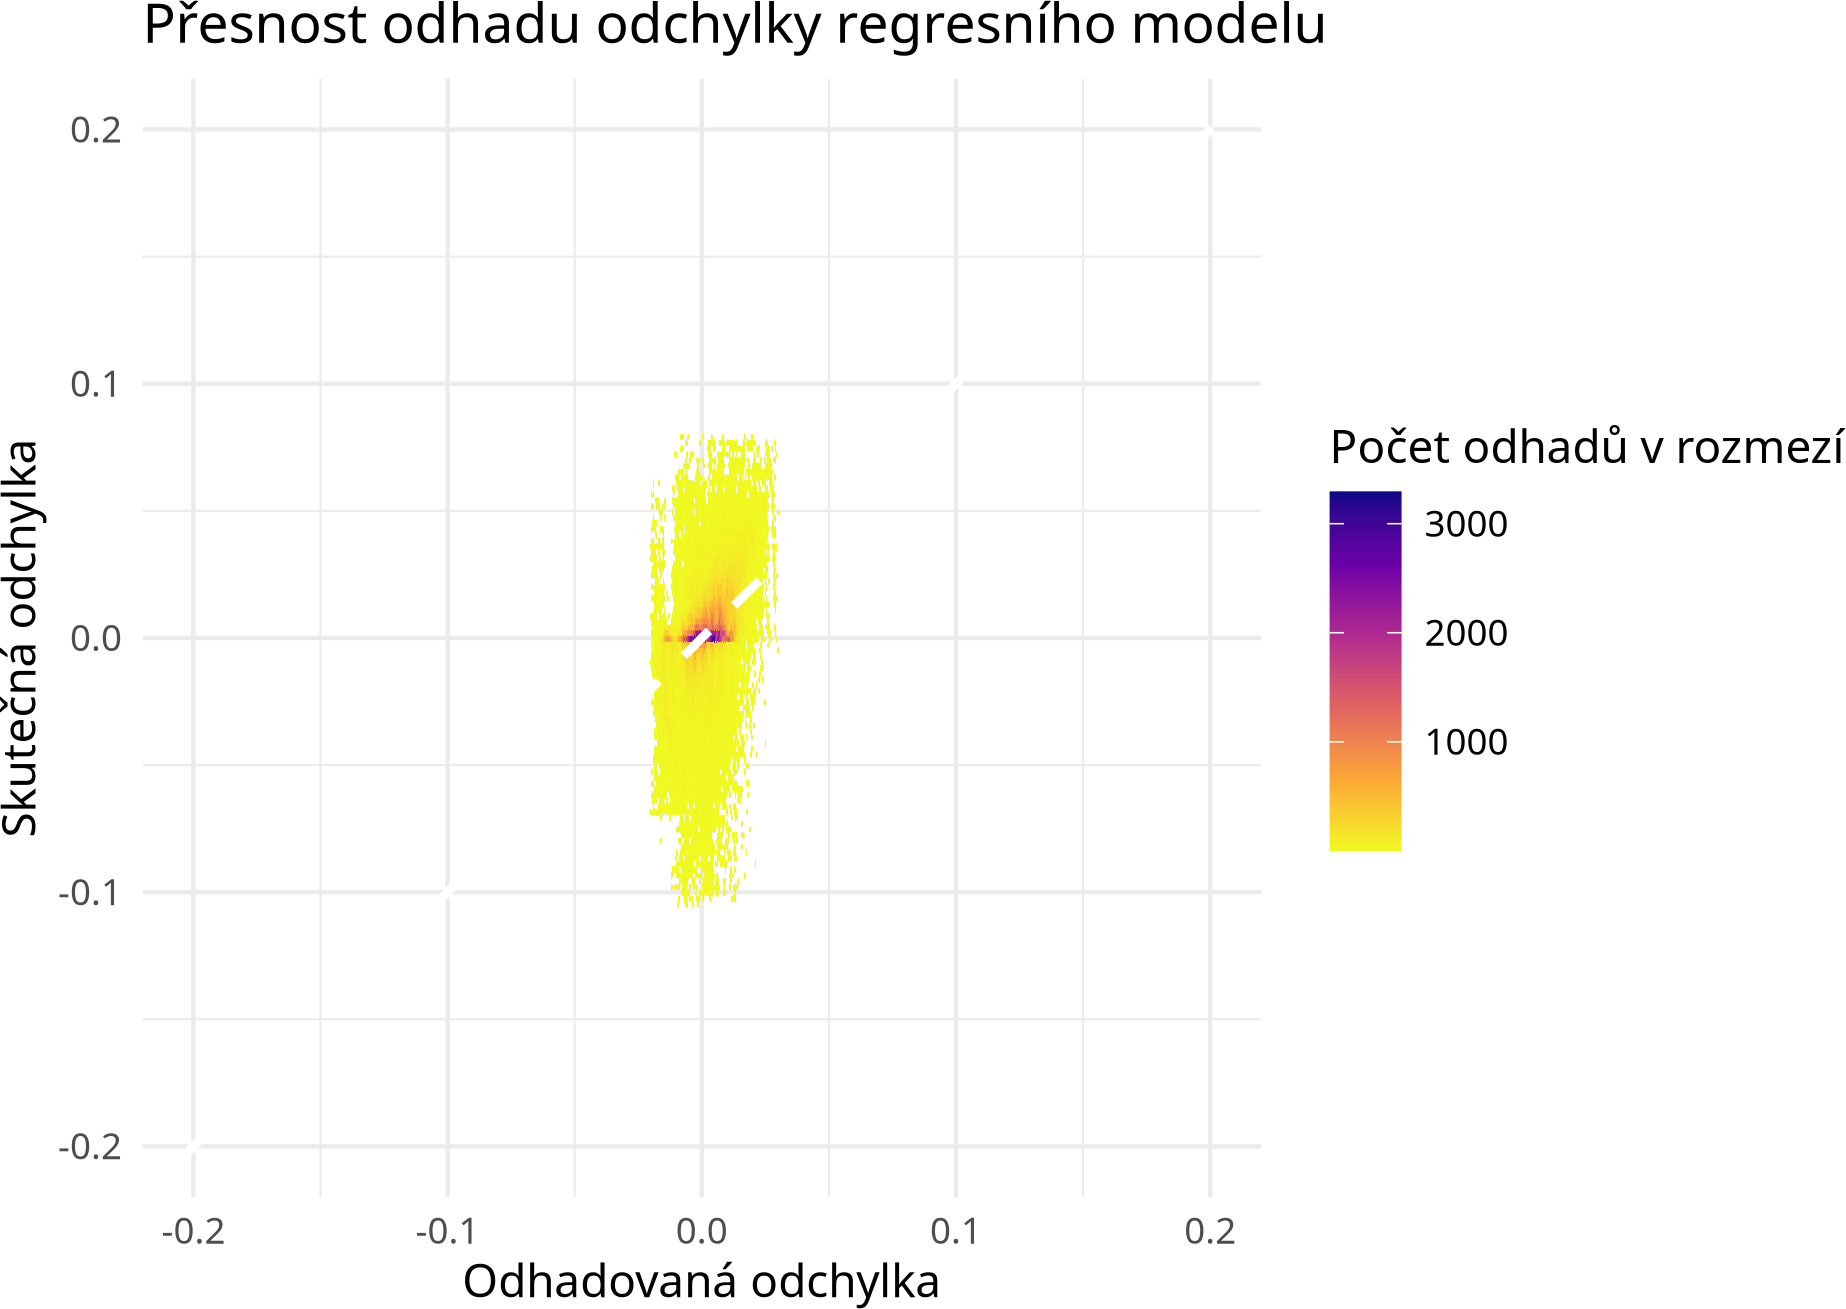
\includegraphics[keepaspectratio]{regression2_files/regression2_files/figure-latex/rmr_post_base_predict_rand3-1.png}}

\begin{Shaded}
\begin{Highlighting}[]
\FunctionTok{anova}\NormalTok{(rmr\_relative)}
\end{Highlighting}
\end{Shaded}

\begin{verbatim}
## Type III Analysis of Variance Table with Satterthwaite's method
##            Sum Sq Mean Sq NumDF  DenDF   F value    Pr(>F)    
## moneyness 0.00488 0.00488     1 328991   17.7251 2.553e-05 ***
## K         0.48015 0.48015     1 318831 1743.7878 < 2.2e-16 ***
## r         1.26289 1.26289     1 328626 4586.5186 < 2.2e-16 ***
## sigma     2.07962 2.07962     1 307205 7552.6721 < 2.2e-16 ***
## q         0.04689 0.04689     1   7947  170.3037 < 2.2e-16 ***
## T         2.30629 2.30629     1 329492 8375.8952 < 2.2e-16 ***
## am_eu     0.00458 0.00458     1     15   16.6244 0.0009689 ***
## call_put  0.72165 0.72165     1 329488 2620.8642 < 2.2e-16 ***
## model     0.00003 0.00001     2 329486    0.0495 0.9517141    
## ---
## Signif. codes:  0 '***' 0.001 '**' 0.01 '*' 0.05 '.' 0.1 ' ' 1
\end{verbatim}

\begin{Shaded}
\begin{Highlighting}[]
\FunctionTok{ranef}\NormalTok{(rmr\_relative)}
\end{Highlighting}
\end{Shaded}

\begin{verbatim}
## $ticker
##         (Intercept)
## ^RUT   0.0200290083
## ^XDA  -0.0245611348
## ^XDB   0.0085831997
## ^XDE  -0.0057006223
## ^XDN   0.0016495493
## AAPL  -0.0124606424
## AMD    0.0124350572
## AMZN  -0.0044011312
## GOOGL  0.0026986683
## JNJ    0.0057295103
## KO    -0.0011771214
## META  -0.0026113541
## MSFT  -0.0036155649
## NFLX  -0.0033547402
## NVDA   0.0036175684
## PG     0.0002661214
## TSLA   0.0028736297
## 
## with conditional variances for "ticker"
\end{verbatim}

--\textgreater{}

\end{document}
